\section*{Ejercicios de tipo test}\label{ejercicios_tipo_test}
\addcontentsline{toc}{section}{Ejercicios de tipo test}

\begin{ejercicio}
Considera el siguiente programa Python:

\begin{python}
def funcion(x):
  # cuerpo
print(funcion(3.5) + 6)
\end{python}

¿Cuál podía ser su cuerpo?:

\begin{choices}
    \choice \pythoninline{return "x"}
    \choice \pythoninline{print(x)}
    \choice \pythoninline{return x} %correct
    \choice \pythoninline{print("x")}
\end{choices}
\end{ejercicio}


\begin{ejercicio}
¿Qué imprime por pantalla el siguiente programa?

\begin{python}
num = 5
def func():
     print(num)
     num = 6
func()
print(num)
\end{python}


\begin{choices}
    \choice 6 \\ 5
    \choice 5 \\ 6
    \choice sale un error %\CorrectChoice
    \choice 6 \\ 6
\end{choices}

\end{ejercicio}

\begin{ejercicio}  ¿Qué es lo que NO forma parte de la cabecera de una función?:

\begin{choices}
    \choice nombre de la función
    \choice valor de retorno   %CORRECT
    \choice lista de parámetros
    \choice palabra clave \texttt{def}
\end{choices}
\end{ejercicio}


\begin{ejercicio} 
Imagine las siguientes instrucciones en Python:

\begin{python}
def hello(x):
    global var
    var+=1
    print(var, x)
var=12
x = var
hello("x")
\end{python}

¿Cuál es el resultado?

\begin{choices}
    \choice \pythoninline{13 x} %CORRECT
    \choice \pythoninline{Error}
    \choice \pythoninline{13 12}
    \choice \pythoninline{13}
\end{choices}

\end{ejercicio}


\begin{ejercicio} Considera el siguiente código Python en el fichero 
\pythoninline{code.py}:

\begin{python}
import pytest
def do_something(s):
  global suma
  suma = 0
  res = "0"
  for i in range(1, len(s)-1):
    if i % 3 == 0:
      suma = suma + int(s[i])
      res = res + s[i]
      print(res)
  return str(suma) + res

@pytest.mark.parametrize("tc_id, entrada, salida_esperada",[
(1, "12345", "404"),
(2, "012345012345", "60303"),
(3, "-1256", "505"),
(4, "", "0")])

def test_values_string(tc_id, entrada, salida_esperada):
    assert do_something(entrada) == salida_esperada
\end{python}

¿Cuál es el resultado cuando llamamos a \pythoninline{\!py.test code.py}?

\begin{choices}
    \choice  1 failed, 3 passed in 0.14s   %CORRECT
    \choice  2 failed, 2 passed in 0.14s
    \choice  3 failed, 1 passed in 0.14s
    \choice  4 passed in 0.14s
\end{choices}

\end{ejercicio}

\begin{ejercicio} Considera el siguiente código Python en el fichero 
\pythoninline{values_string.py}:

\begin{python}
import pytest

def values_string(s):
  result = "" 
  for i in range(len(s)):
    if i % 2 == 0:
      result = result + s[i]
  return result

@pytest.mark.parametrize("tc, entrada, salida",[
(1, "12345", "135"),
(2, "01234567", "1357"),
(3, "-112241", "-11"),
(4, "", "")])

def test_values_string(tc, entrada, salida):
    assert values_string(entrada) == salida, "caso {0}".format(tc)
\end{python}

¿Cuál es el resultado cuando llamamos a \pythoninline{\!py.test values_string.py}?

\begin{choices}
    \choice  2 failed, 2 passed in 0.14s %CORRECT
    \choice  1 failed, 3 passed in 0.14s
    \choice  3 failed, 1 passed in 0.14s
    \choice  4 passed in 0.14s
\end{choices}


\end{ejercicio}


\begin{ejercicio}  Considera el siguiente programa Python:

\begin{python}
def func(y, x = 1):
    y = 2
    x = x + y
    y += 1
    print(x)
\end{python}

¿Qué imprime cuando llamamos a \verb|func(4)|?

\begin{choices}
    \choice 3   %CORRECT
    \choice 6
    \choice 7
    \choice 4
\end{choices}

\end{ejercicio}

\begin{ejercicio} Considera los siguientes tests y test driver:

\begin{small}
\begin{python}
@pytest.mark.parametrize("n, a, b, c, o",[
(1, 3, [3,5], 2.4, "hola"),
(2, 5, "a", 3.0, "onetwoone")
])
def test_funcionX(n, a, b, c, o):
    assert funcionX(a, b, c) == o,  "test {0}".format(n)
\end{python}
\end{small} 

Considerar también las siguientes funciones:

\begin{small}
\begin{python}
def funcion1(a):
    print("hola")

def funcion2 (a, b):
    return "hi" + a + b

def funcion3(a, b, c):
    return str(a) + "onetwoone"

def funcion4 (a, b, c, d):
    return "hola"
\end{python}
\end{small} 

El driver \pythoninline{test_funcionX} solo puede ser para testear la \pythoninline{funcionX} con X igual a:

\begin{choices}
    \choice 3   %CORRECT
    \choice 1
    \choice 2
    \choice 4
\end{choices}
\end{ejercicio}



\begin{ejercicio} Mira el siguiente esquema con las cajas numeradas.

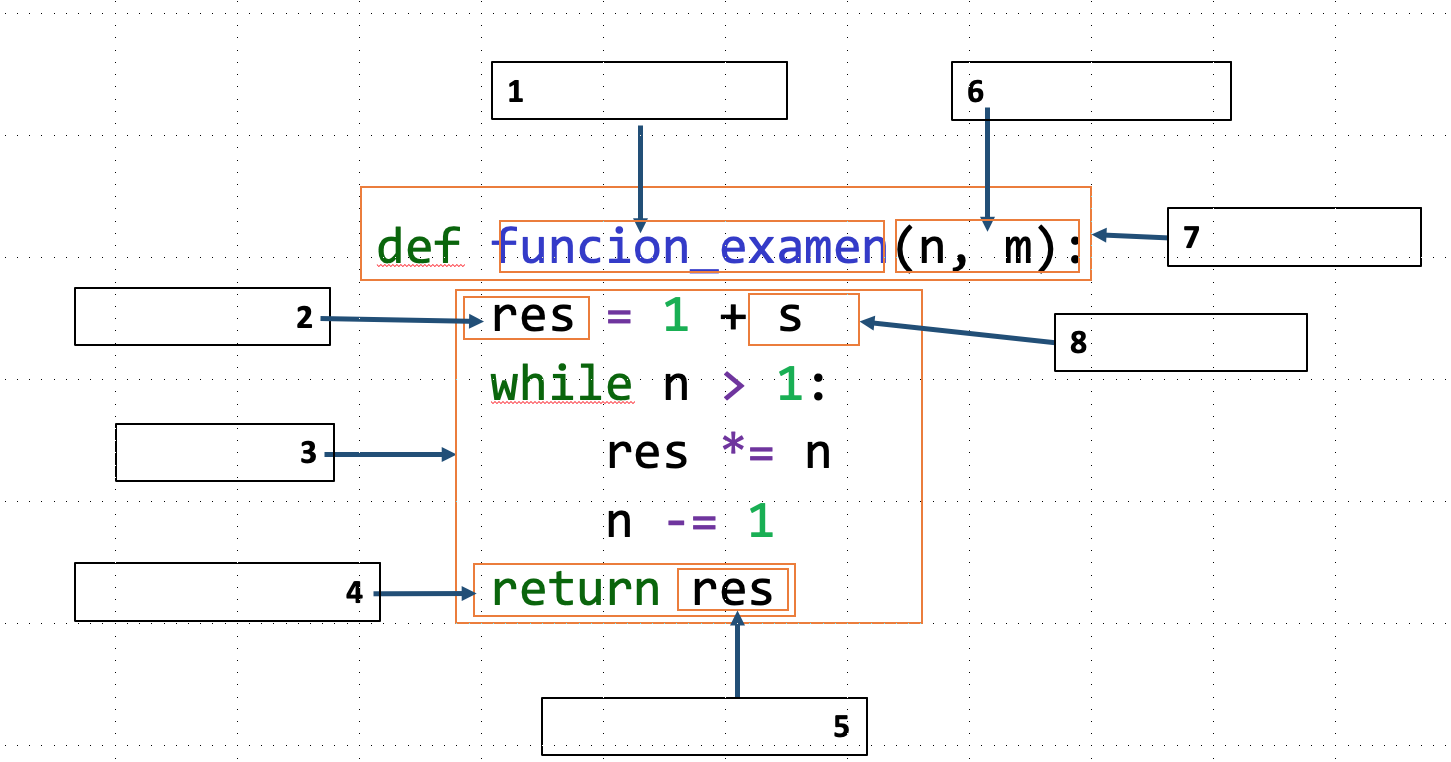
\includegraphics[width=0.5\textwidth]{book/Spanish/05_Funciones/images/funcion.png}

¿Cuál de los siguientes es correcto?

\begin{choices}
    \choice caja 1 contiene el nombre de la función, res es una variable local, caja 3 contiene el cuerpo, caja 6 tiene los parametros   %CORRECT
    \choice caja 1 representa la cabecera, n es una variable global, cajita 3 contiene el cuerpo, s es una variable global
    \choice cala 4 contiene la instrucción de retorno, caja 5 contiene el valor devuelto, variables n y m siempre tiene que ser global  
    \choice res es una variable global, caja 4 contiene la instrucción de retorno, caja 5 contiene el valor devuelto, s es una variable local

\end{choices}
\end{ejercicio}

